\documentclass[c]{beamer}

\usepackage[utf8]{inputenc}
\usepackage[french]{babel}

\usepackage{amsmath}
\usepackage{amsfonts}
\usepackage{amsthm}

\newtheorem*{deffr}{Définition}
\newtheorem*{propriete}{Propriété}
\newtheorem*{theofr}{Théorème}

\usetheme{Warsaw}

\title{Détection de communautés et génération de graphes}
\author{Igor Colin}
\date{\today}

\setbeamertemplate{navigation symbols}{}

\AtBeginSection[]
{
    \begin{frame}<beamer>
        \tableofcontents[currentsection]
    \end{frame}
}

\begin{document}

\maketitle

\section{Détection de communautés}
\begin{frame}

    \begin{itemize}
        \item Approche spectrale
        \begin{itemize}
            \item Définition d'une mesure de qualité d'une partition d'un
            graphe
            \item Maximisation de cette quantité pour trouver la partition
            optimale
        \end{itemize}

        \begin{figure}
            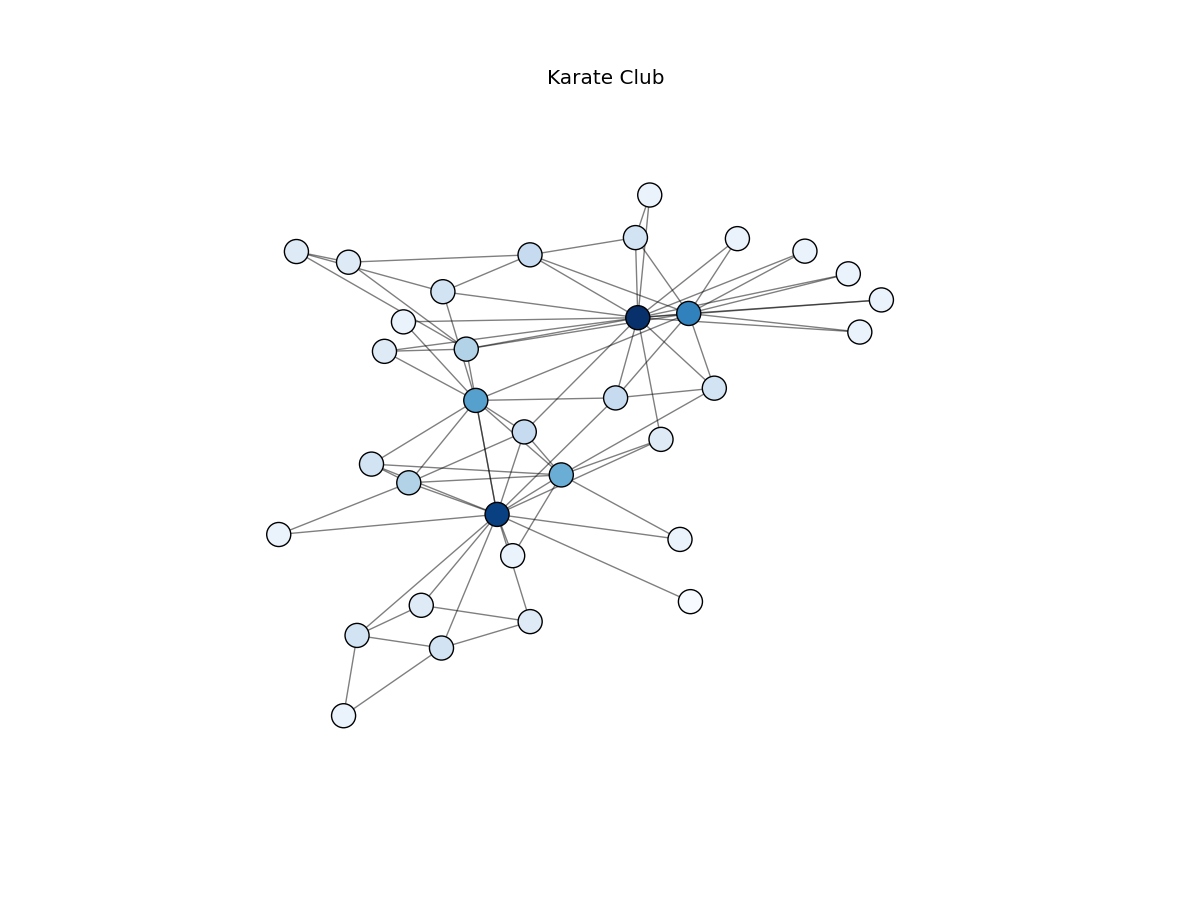
\includegraphics[width=.6\textwidth]{./karate_club.png}
            \caption{Exemple du club de karaté de Zachary.}
        \end{figure}
    \end{itemize}
\end{frame}

\begin{frame}
    \begin{itemize}
        \begin{deffr}
            Soit $G = (V, E)$ un graphe non-orienté et soit $(S, T)$ une
            partition de $V$. La modularité associée à la partition $(S, T)$
            correspond taux d'arrêtes de $E$ contenues dans $S$ ou $T$ comparé
            au taux d'arrêtes qui auraient été contenues dans $S$ ou $T$ si
            l'on avait distribué les arrêtes du graphe aléatoirement.
        \end{deffr}

        \item Définition de la modularité dépendantes de l'aléa autorisé sur
        les arrêtes
        \item Approche usuelle : degrés des n\oe{}uds conservés
    \end{itemize}

\end{frame}

\begin{frame}

    \begin{deffr}
        Soit $G = (V, E)$ un graphe non-orienté et soit $(S, T)$ une partition
        de $V$. On note $\mathbf{A}$ la matrice d'adjacence associée à $G$.
        Sous les conditions précédentes, la modularité $Q(S, T)$ peut-être
        exprimée sous la forme suivante :
        \[
            Q(S, T) = \frac{1}{2|E|} \sum_{(i, j) \in V \times V}
                \left( A_{ij} - \frac{d_i d_j}{2|E|} \right)
                \mathbf{1}_{\{s_i = s_j\}},
        \]
        où, pour tout $k \in V$,
        \[
            s_k = \left\{
                \begin{array}{ll}
                    +1 & \text{si $k \in S$} \\
                    -1 & \text{si $k \in T$}
                \end{array}
            \right.
        \]
    \end{deffr}

Remarque : $Q(V, \emptyset) = 0$

\end{frame}

\begin{frame}

    \begin{deffr}
        Soit $G = (V, E)$ un graphe non-orienté et soit $\mathbf{A}$ la matrice
        d'adjacence associée. On note $\mathbf{D} = \mathbf{diag}\left((d_i)_{i \in V}\right)$.
        La matrice de Laplace normalisée $\mathbf{L}$ associée au graphe $G$ est
        définie par :
        \[
            \mathbf{L} = \mathbf{D}^{-1/2} \mathbf{A} \mathbf{D}^{-1/2}.
        \]
    \end{deffr}

    \begin{theofr}
        Soit $G = (V, E)$ un graphe non-orienté. Soit $\mathbf{u^{(2)}}$ le vecteur
        propre associé à la deuxième plus grande valeur propre de la matrice de
        Laplace normalisée. Alors la partition $(S, T)$ définie par :
        \[
            \left\{
                \begin{array}{r c l}
                    S & = & \{ i \in V \text{, } u^{(2)}_i > 0 \} \\
                    T & = & \{ i \in V \text{, } u^{(2)}_i \leq 0 \}
                \end{array}
            \right. ,
        \]
        est solution non triviale du problème de maximisation de la modularité.

    \end{theofr}

\end{frame}

\begin{frame}
    \begin{figure}
        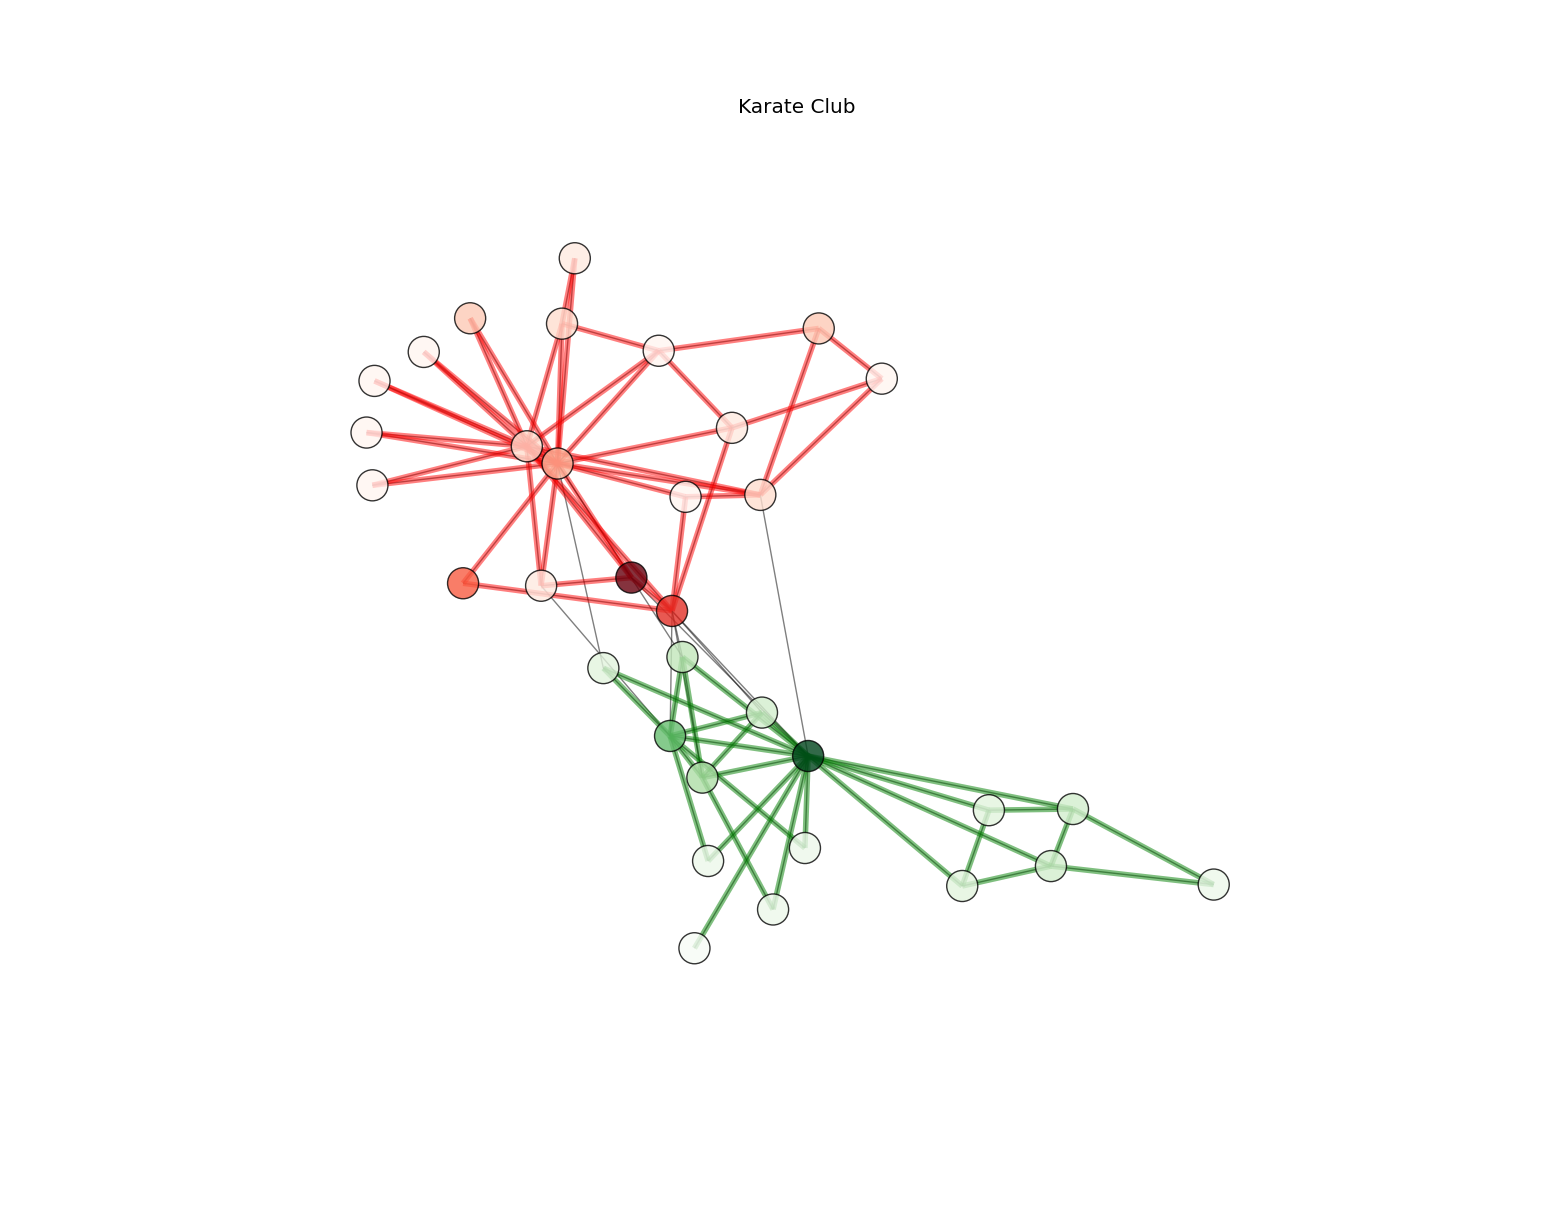
\includegraphics[width=.8\textwidth]{./karate_club_split.png}
        \caption{Détection de communauté appliquée au club de karaté de
        Zachary.}
    \end{figure}
\end{frame}

\begin{frame}
    \begin{itemize}
        \item Méthode simple à implémenter
        \item Critère interprétable
        \item Limites : coût en $\mathcal{O} (|V|^3)$
        \item Nécessité d'utiliser une méthode adaptée pour de grands réseaux
    \end{itemize}
\end{frame}

\begin{frame}
    Méthodes randomisées
\end{frame}

\section{Génération de graphe}

\begin{frame}
    \begin{itemize}
        \item Actuellement, peu d'utilisateurs sur l'application
        \item Nécessité de créer des graphes plus grands pour tester les
            méthodes employées
        \item Comment générer des graphes capable de \og prédire \fg{} le
            futur de l'application ?
    \end{itemize}
\end{frame}

\begin{frame}
    \begin{itemize}
        \item MCMC
        \begin{itemize}
            \item Switching : degré, degré joint
            \item Matching
            \item Garantie d'indépendance
        \end{itemize}
        \item Social, épidémiologique, etc.
        \begin{itemize}
            \item Attachement préférentiel
            \item Kronecker
            \item Forest fire
        \end{itemize}
    \end{itemize}
\end{frame}

\end{document}
